% !TeX root = ../main.tex
\appendix
\setcounter{figure}{0}
\renewcommand{\thefigure}{\Alph{section}.\arabic{figure}}
\makeatletter
\if@firstcolumn\else\newpage\fi
\makeatother
\par\smallskip
\noindent\makebox[0pt][l]{%
\begin{minipage}{\textwidth}
\section{Additional qualitative results on test cases}
\label{app:additional_qualitative}

\textcolor{red}{This appendix presents additional qualitative comparisons on test cases. In each row, the engineer-designed reference, the room-based prediction, and the edge-based baseline are shown from left to right. The six rows include two cases from each condition group, covering low-, medium-, and high-density layouts. These additional cases further show that the proposed room-based method generally produces more coherent and boundary-aligned shear wall layouts than the edge-based baseline. They also reveal remaining local errors in some predictions, such as overly short shear wall segments or missing walls in detailed regions, indicating that fine-grained local refinement remains a direction for future improvement.}
\end{minipage}}
\par\smallskip

\begin{figure*}[!t]
\centering
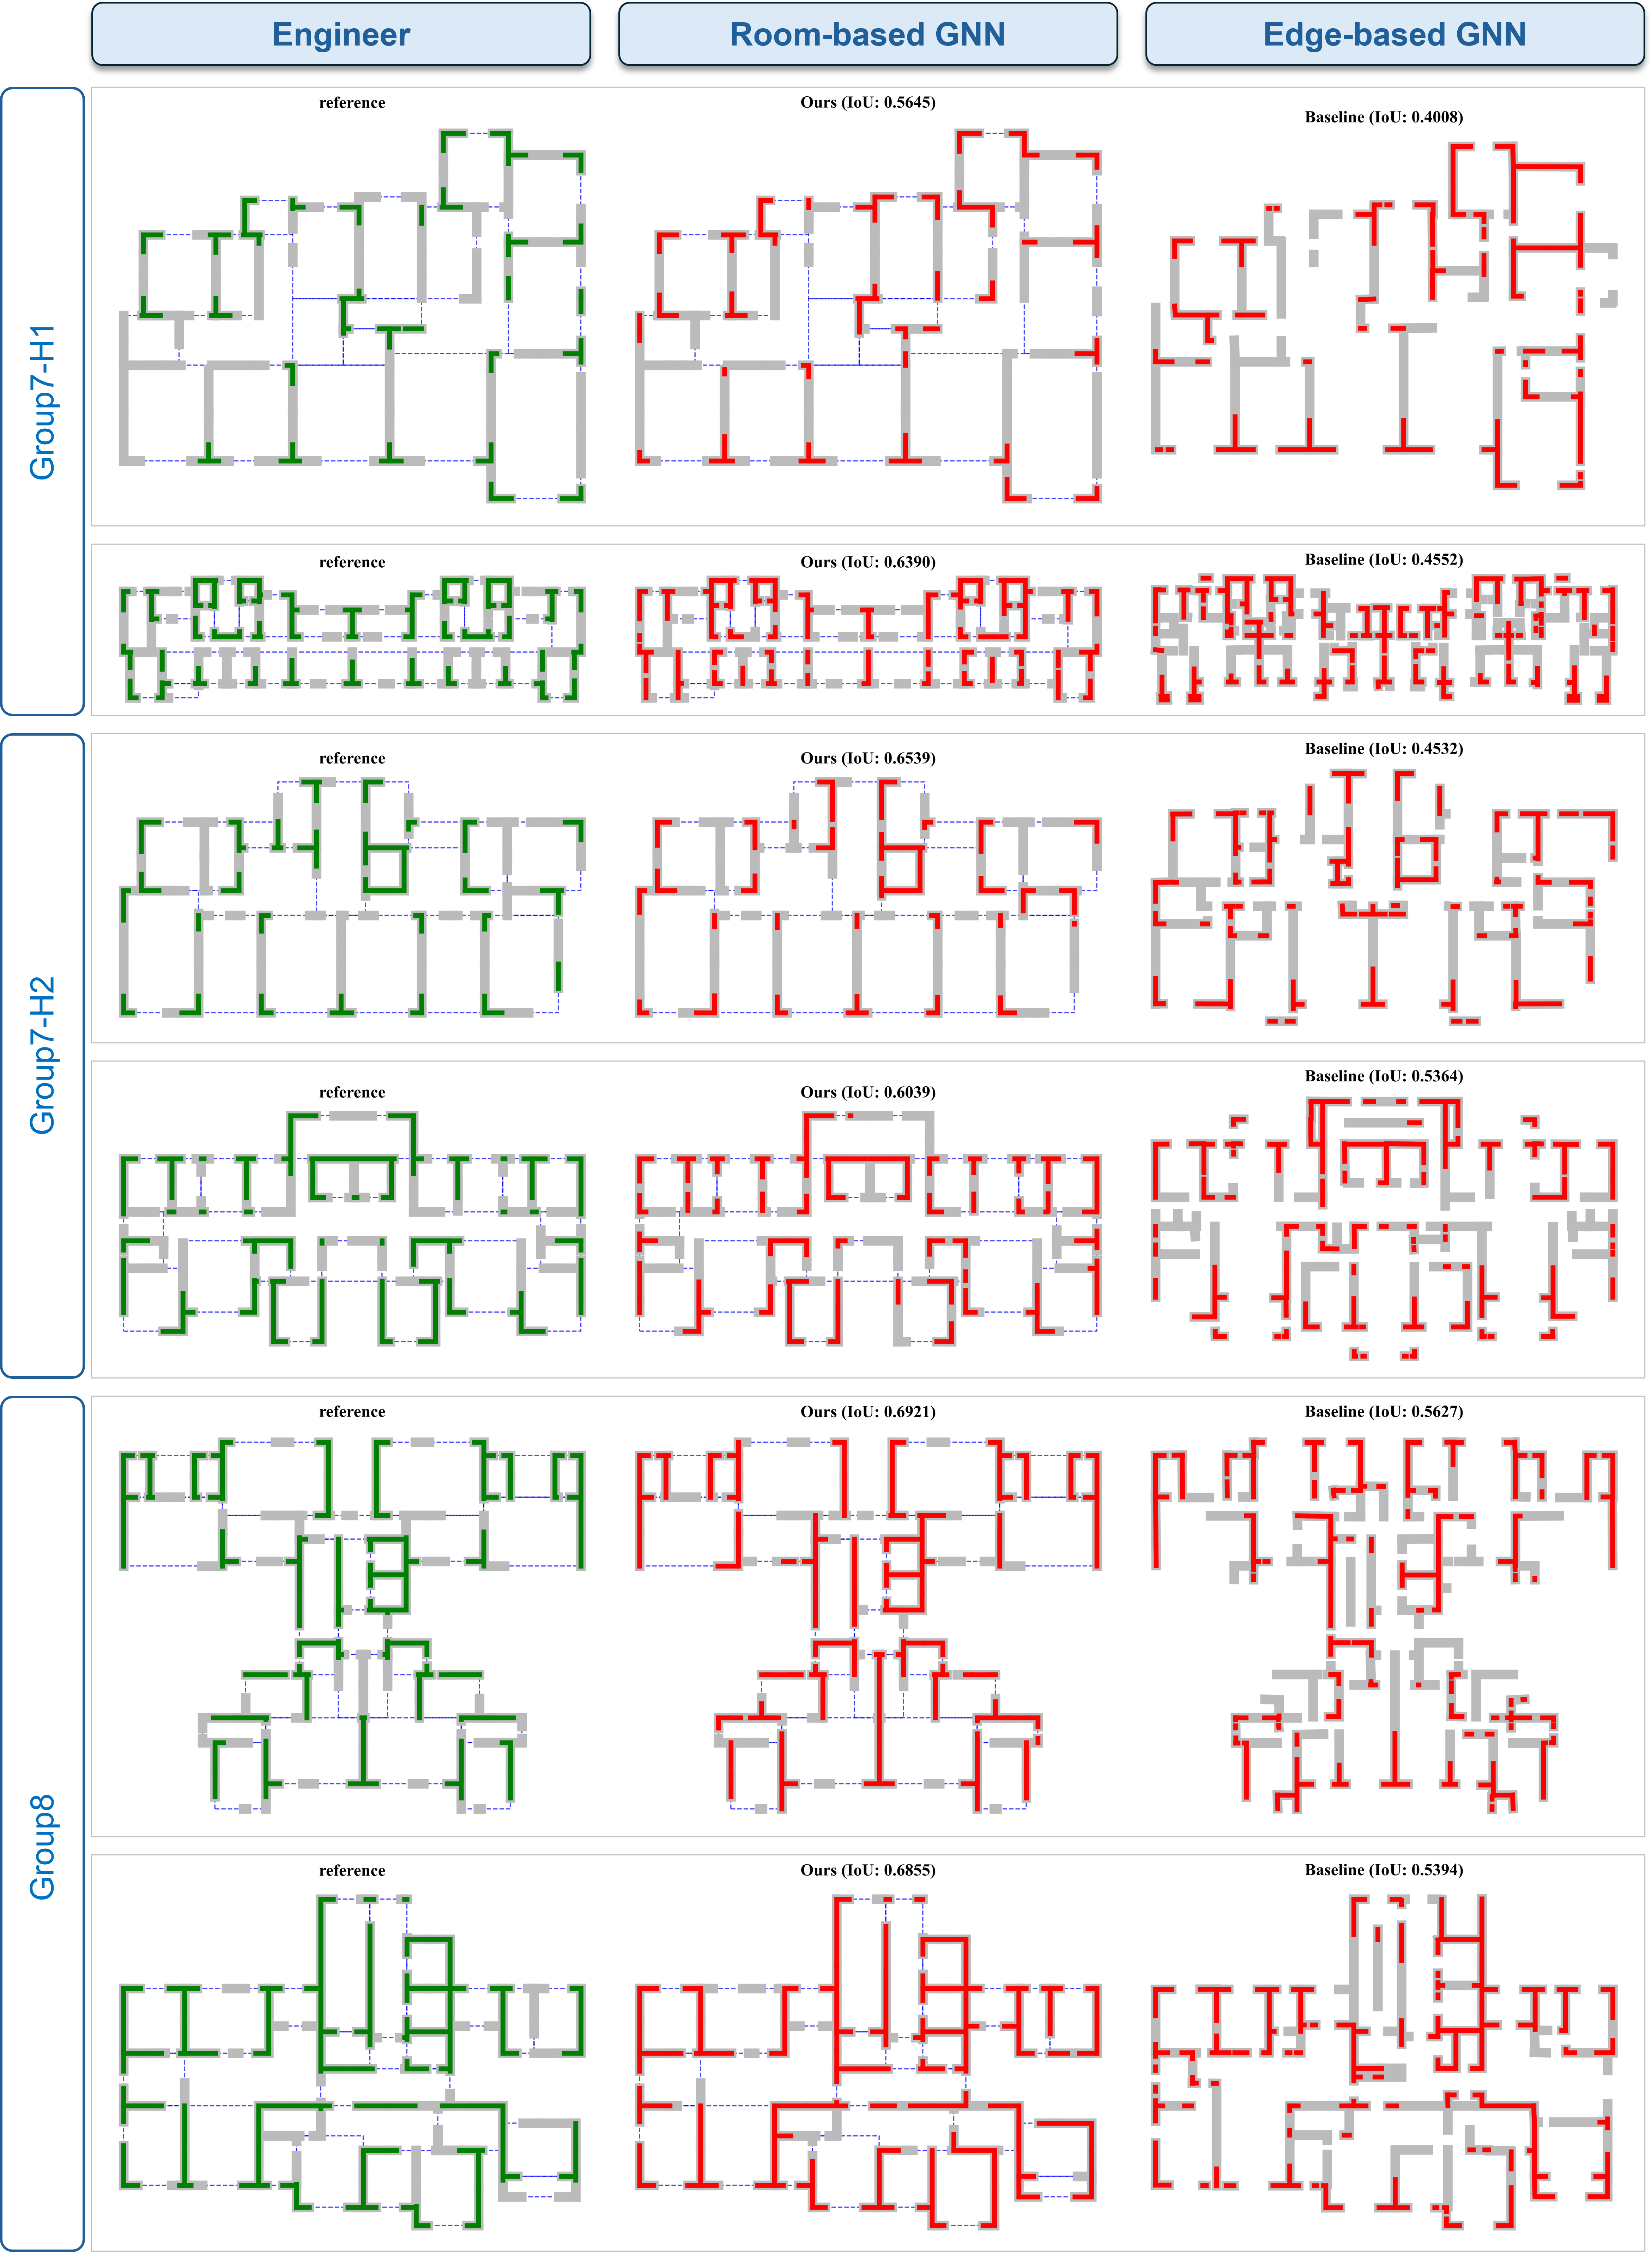
\includegraphics[width=\textwidth,height=0.82\textheight,keepaspectratio]{supp_case.png}
\caption{\textcolor{red}{Additional qualitative comparisons on test cases. Each row shows the engineer-designed layout, the room-based prediction, and the edge-based baseline. The six examples include two layouts from each condition group.}}
\label{fig:supp_case}
\end{figure*}
